\documentclass{article}
%% PACKAGES %%

\usepackage{amsmath, amsfonts, amssymb, amsthm}
\usepackage{braket}
\usepackage{listings}
\usepackage{geometry}
\usepackage{xcolor}
\usepackage{textcomp}
\usepackage{graphicx}
\usepackage{fancyhdr}
\usepackage{sourcecodepro}
\usepackage{multirow}

%%%%%%%%%%%%%%

\graphicspath{{./images}}
\setlength\parindent{0pt}       % globally supress indentation

%% LISTINGS CONFIG %%

\definecolor{purple2}{RGB}{153,0,153} % there's actually no standard purple
\definecolor{green2}{RGB}{0,153,0} % a darker green

\lstset{
  language=MATLAB,                   % the language
  basicstyle=\normalsize\ttfamily,   % size of the fonts for the code
  frame = single,
  % Color settings to match IDLE style
  keywordstyle=\color{orange},       % core keywords
  keywordstyle={[2]\color{purple2}}, % built-ins
  stringstyle=\color{green2},%
  showstringspaces=false,
  commentstyle=\color{red},%
  upquote=true,                      % requires textcomp
  numbers=left,
  breaklines=true,
}

% Title Stuff
\title{\vspace{-3cm}ECE355L Project 2}
\author{Chase A. Lotito, \textit{SIUC Undergraduate}}
\date{}

\begin{document}

\pagestyle{fancy}

% attempt to make nice header
\fancyhead{}
\fancyhead[CH]{\normalsize{LOTITO --- ECE355L --- PROJECT 2}}

\maketitle % Makes the title

\section{Exercise 1}

We are given the following differential equation with initial conditions, \(y(0)=1\), \(y'(0) = 1\), and \(y''(0)=0\):

\begin{equation} 
    y''' + 8y'' + 2521y' + 5018y = f'' + 5018f
\end{equation}

We can solve for a symbolic expression of \(y\) using the \textit{dsolve} method which is apart of the Symbolic Math Toolbox extension in MATLAB. This requires us to create a symbolic character variable for \(y(t)\), then using the \textit{diff} method to differentiate our signals as necessary.

\begin{lstlisting}
% Chase Lotito - SIUC - Spring 2024
% ECE355L - Project 2
% Q1: dsolve to solve for zero-input response
% y0 = dsolve('D3y + 8*D2y + 2521*Dy + 5018*y = 0', 'y(0)=1', 'Dy(0)=1', 'D2y(0)=0');

% system variable
syms y(t)           % make y a function of t

% initial conditions
Dy = diff(y,t);         % define D operator
D2y = diff(y,t,2);      % define D2 operator
cond = [y(0) == 1, Dy(0) == 1, D2y(0) == 0]; % set initial conditions

y0 = diff(y, t, 3) + 8 * diff(y, t, 2) + 2521 * diff(y, t) + 5018 * y == 0;
S = dsolve(y0, cond); % solve diff eq. with ICs

% get latex of it
chr = latex(S);
\end{lstlisting}

In the "Command Window":

\begin{lstlisting}
S =
 
(exp(-3*t)*(7489*sin(50*t) - 700*cos(50*t) + 125750*exp(t)))/125050
\end{lstlisting}

The code also provides us a symbolic LaTeX equivalent for \(y_0(t)\) in \(chr\):

\begin{equation}
   y_0(t) = \frac{{\mathrm{e}}^{-3\,t}\,\left(7489\,\sin\left(50\,t\right)-700\,\cos\left(50\,t\right)+125750\,{\mathrm{e}}^t\right)}{125050} 
\end{equation}

\clearpage

\section{Exercise 2}

We can then plot the zero-input response for the system in the previous exercise via this additional code. Here \textit{fplot} is a function in provided by Symbolic Math Toolbox that plots symbolic expressions:

\begin{lstlisting}
% ... Exercise 1 Code Above...
fplot(S, [0,4]);    % fplot(<function>, [<xmin>, <xmax>])
xlabel('t');
ylabel('y0(t)');
title('Zero-Input Response');
\end{lstlisting}

Remember that from Exercise 1, \(S\) was set equal to the symbolic expression for \(y_0(t)\). Then we get the following plot:

\begin{figure}[!ht] 
    \centering
    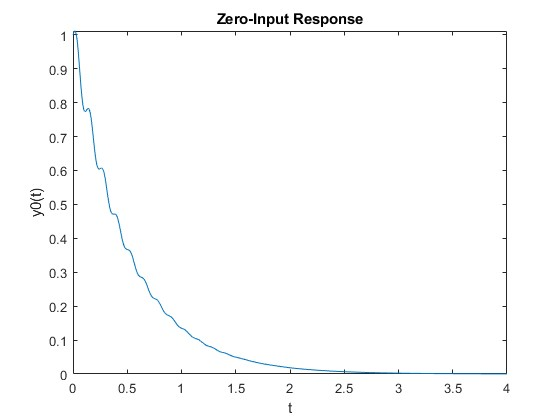
\includegraphics[width = 10cm]{q2.jpg}
    \caption{Zero-Input response of system}
    \label{fig:zeroinput}
\end{figure}

\section{Exercise 3}

Create a system object using \(tf\) for the system from part 1 and obtain the zero-state impulse and step response using impulse and step function.

\bigskip

\textbf{Solution.}

\bigskip

Again, here is the differential equation that describes our system (w.r.t. time):

\begin{equation} 
    y''' + 8y'' + 2521y' + 5018y = f'' + 5018f
\end{equation}

To get to the transfer function, we need to take the Laplace transform, omitting any initial conditions:


\begin{equation} 
    s^3 Y(s) + 8s^2 Y(s) + 2521s Y(s) + 5018 Y(s) = s^2 F(s) + 5018 F(s)
\end{equation}

This we can rearrange to get the transfer function \(H(s)\):

\begin{equation}
    H(s) = \frac{Y(s)}{F(s)} = \frac{s^2 + 5018}{s^3 + 8 s^2 + 2521 s + 5018}
\end{equation}

Using the Control Systems Toolbox extension in MATLAB, we can take the numerator and denominator of \(H(s)\) and solve for the step and impulse responses.

\begin{lstlisting}
% Chase Lotito - 355L Project 2 - Exercise 3
% Define the numerator and denominator coefficients
num = [1 0 5018];
den = [1 8 2521 5018];
% Create the transfer function object
TFsys = tf(num, den);
% Remove the roots from the transfer function
TFsys_no_roots = tzero(TFsys);
% Define the time vector
t_vec = 0:0.01:10; % Time vector from 0 to 10 with a step size of 0.01
% Calculate the step response
[ystep, t_step] = step(TFsys_no_roots, t_vec);
% Calculate the impulse response
[h, t_impulse] = impulse(TFsys_no_roots, t_vec);
% Plot the step response
subplot(2, 1, 1);
plot(t_vec(1:length(ystep)), ystep); % Adjust the length of t_vec
title('Step Response');
xlabel('t');
ylabel('y_{step}(t)');
% Plot the impulse response
subplot(2, 1, 2);
\end{lstlisting}

\begin{figure}[!ht] 
    \centering
    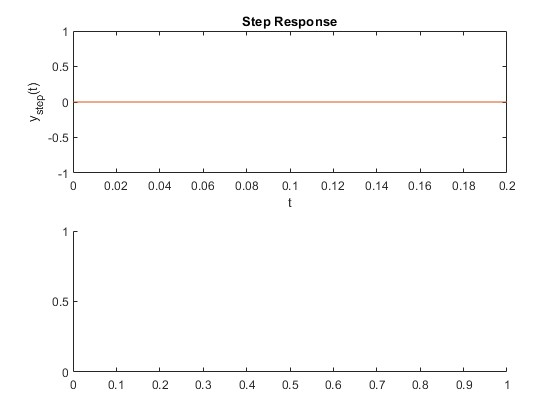
\includegraphics[width = 10cm]{q3.jpg}
    \caption{Step-Response and Impulse-Response}
    \label{fig:q3}
\end{figure}



\end{document}
